
\newcommand{\tikzI}{
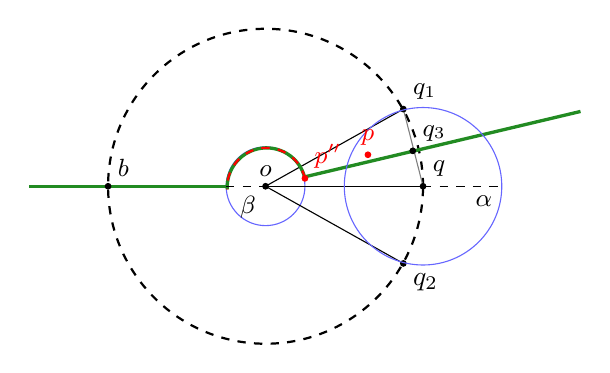
\begin{tikzpicture}
    %color for special region
    %\foreach \ang/\col in {3/gray} {
    %  \fill[\col!20] (74+100*\ang:2)--(0,0)--(30+90*\ang+90:2)--cycle;  }
    % Ball(i*,1)
    \draw[color=black,  dashed, thick](0,0) circle (2);
    % Ball(o,beta)
    \draw[color=blue!60, inner color=white, thin](0,0) circle (0.5);
    \filldraw[black] (0,0) circle (1pt) node[anchor=south ]{\small $o$};
    \draw[black, thin] (0,0) -- (2,0) ;
   % \draw[red, thick] (1.75,0.94) arc (34.8:12.6:1.3);
    
    %lines 
    \draw[black, thin] (0,0) -- (1.75,0.98) ;
    \draw[black, thin] (0,0) -- (1.75,-0.98) ;

    \draw[ForestGreen, very thick] (0.5,0.12) -- (4,0.95) ;
    \draw[ForestGreen, very thick] (-0.5,0) -- (-3,0) ;
    \draw[ForestGreen, very thick] (0.5,0.10) arc (13:183:0.5);
    \draw[black!50] (2,0) -- (1.75,0.98) ;
    \filldraw[black] (1.75,0.98) circle (1pt) node[anchor=south west ]{\small \small $q_1$};
    \filldraw[black] (1.75,-0.98) circle (1pt) node[anchor=north west  ]{$q_2$};
    \draw[black, dashed] (-0.5,0) -- (0,0) node[anchor=north east ]{\small $\beta$};
    \draw[red, thick, dashed] (0.5,0.10) arc (13:183:0.5);
    \filldraw[red] (0.5,0.10) circle (1pt) node[anchor=south west]{\small$p''$};
    % Ball(i',alpha)
    \draw[color=blue!60, thin](2,0) circle (1);
    \filldraw[black] (2,0) circle (1pt) node[anchor=south west]{\small$q$};
    \filldraw[black] (1.87, 0.45) circle (1pt) node[anchor=south west]{\small$q_3$};

    \draw[black, dashed] (2,0) -- (3,0) node[anchor=north east ]{ \small $\alpha$};
    % point(i)
    \filldraw[black] (-2,0) circle (1pt) node[anchor=south west]{\small $b$};
    % point(j)
    \filldraw[red] (1.3,0.40) circle (1pt) node[anchor=south]{\small $p$};
    \end{tikzpicture}
}

\newcommand{\tikzII}{
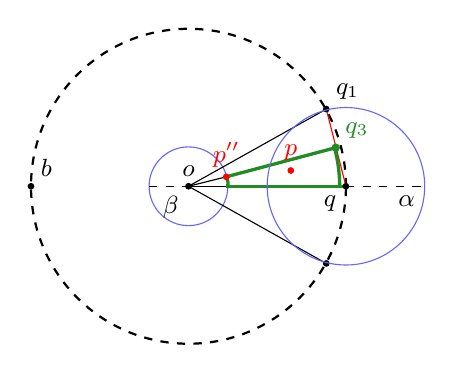
\begin{tikzpicture}
    %color of special region
    %\foreach \ang/\col in {3/gray} {
         %  \fill[\col!20] (60+100*\ang:2)--(0,0)--(15+90*\ang+90:2)--cycle;  }
    % Ball(i*,1)
    \draw[color=black,  dashed, thick](0,0) circle (2);
    % Ball(i*,beta)
    \draw[color=blue!60,inner color=white, thin](0,0) circle (0.5);
    % point(i)
    \filldraw[black] (-2,0) circle (1pt) node[anchor=south west]{\small $b$};
    \draw[black, dashed] (-0.5,0) -- (0,0) node[anchor=north east ]{\small $\beta$};
    \filldraw[black] (0,0) circle (1pt) node[anchor=south ]{\small $o$};
    \draw[black, thin] (0,0) -- (2,0) ;
    %lines 
    \draw[black, thin] (0,0) -- (1.75,0.98) ;
    \draw[black, thin] (0,0) -- (1.75,-0.98) ;
    \draw[ForestGreen, very thick] (0.48,0.12) -- (1.87,0.49) ;
    \draw[red, thin] (1.75,0.98) -- (2,0) ;
    %\draw[ForestGreen, very thick] (1.87,0.49) -- (2,0) ;
    \draw[ForestGreen, very thick] (0.48,0) -- (2,0) ;
    \draw[ForestGreen, very thick] (1.92,0) arc (0:15.8:1.87);
    \draw[ForestGreen, very thick] (0.48,0.12) arc (28.2:-11.6:0.2);
    % point p_1
    \filldraw[black] (1.75,0.98) circle (1pt) node[anchor=south west ]{\small \small $q_1$};
    %point p_3
    \filldraw[ForestGreen] (1.87,0.49) circle (1.3pt) node[anchor=south west ]{\small \small $q_3$};
    \filldraw[black] (1.75,-0.98) circle (1pt) node[anchor=south west ]{};
    % j'
    \draw[black] (0,0)--(0.48,0.12);
    \filldraw[red] (0.48,0.12) circle (1pt) node[anchor=south ]{\small $p''$};
    % Ball(x',alpha)
    \draw[color=blue!60, thin](2,0) circle (1);
    \filldraw[black] (2,0) circle (1pt) node[anchor=north east]{\small$q$};
    \draw[black, dashed] (2,0) -- (3,0) node[anchor=north east ]{ \small $\alpha$};
    % point(p)
    \filldraw[red] (1.3,0.20) circle (1pt) node[anchor=south]{\small $p$};
    \end{tikzpicture}
}

\newcommand{\tikzIII}{
    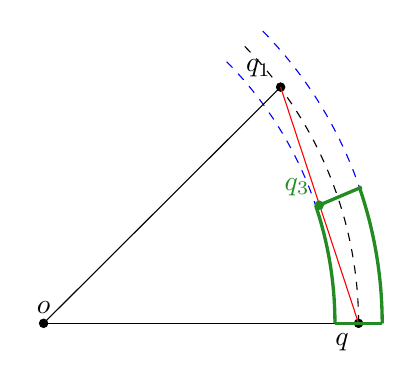
\begin{tikzpicture}
        \draw[dashed, blue] (-0.3,0) arc (0:45:4.7);
        \draw[dashed, blue] (0.3,0) arc (0:45:5.3);
        \draw[dashed, black] (0,0) arc (0:45:5);
        \filldraw[black] (-4,0) circle (1.5pt) node[anchor=south]{ $o$};
        \filldraw[black] (0,0) circle (1.5pt) node[anchor=north east]{ $q$};
        \filldraw[black] (-0.99,3) circle (1.5pt) node[anchor=south east]{ $q_1$};    
        \draw[black] (0,0) -- (-4,0);
        \draw[black] (-4,0) -- (-0.99,3);
        \draw[red] (0,0) -- (-0.99,3);
        \filldraw[ForestGreen] (-0.5,1.5) circle (1.5pt) node[anchor=south east]{ $q_3$}; 
        \draw[ForestGreen, very thick] (0.3,0) arc (0:18.8:5.3);
        \draw[ForestGreen, very thick] (-0.3,0) arc (0:18.5:4.7);
        \draw[ForestGreen, very thick] (-0.5,1.5) --(0.04 , 1.73);
        %\draw[black] (0.5,1.93) -- (-4,0);
        \draw[ForestGreen, very thick] (-0.3,0) -- (0.3,0);
    \end{tikzpicture}
}

\newcommand{\tikzIV}{
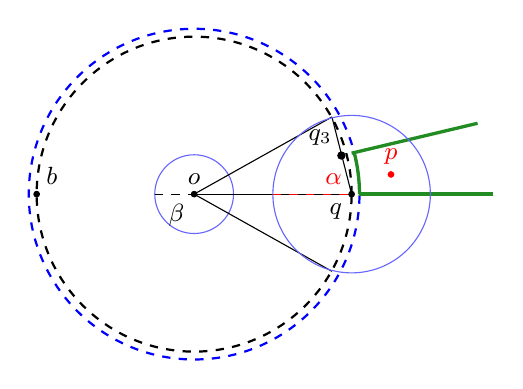
\begin{tikzpicture}
    %color of special region
    %\foreach \ang/\col in {3/gray} {
         %  \fill[\col!20] (60+100*\ang:2)--(0,0)--(15+90*\ang+90:2)--cycle;  }
    % Ball(i*,1)
    \draw[color=black,  dashed, thick](0,0) circle (2);
    \draw[color=blue,  dashed, thick](0,0) circle (2.1);
    % Ball(i*,beta)
    \draw[color=blue!60,inner color=white, thin](0,0) circle (0.5);
    % point(i)
    \filldraw[black] (-2,0) circle (1pt) node[anchor=south west]{\small $b$};
    \draw[black, dashed] (-0.5,0) -- (0,0) node[anchor=north east ]{\small $\beta$};
    \filldraw[black] (0,0) circle (1pt) node[anchor=south ]{\small $o$};
    \draw[black, thin] (0,0) -- (2,0) ;
    %lines 
    \draw[black, thin] (0,0) -- (1.75,0.98) ;
    \draw[black, thin] (0,0) -- (1.75,-0.98) ;
    %\draw[black, thin] (0.48,0.12) -- (2.7,0.7) ;
    \draw[ForestGreen, very thick] (2,0.52) -- (3.6,0.9) ;
    \draw[ForestGreen, very thick] (2.1,0) -- (3.8,0) ;

    %\draw[ForestGreen, very thick] (3,0) arc (0:48.5:1);
    \draw[ForestGreen, very thick] (2.1,0) arc (0:15:2.1);
    \draw[black, thin] (1.75,0.98) -- (2,0) ;
    \filldraw[red] (2.5,0.25) circle (1pt) node[anchor=south ]{\small $p$};
    % point p_1

    %point p_3
    \filldraw[black] (1.87,0.49) circle (1.3pt) node[anchor=south east ]{\small $q_3$};

 
    % Ball(i',alpha)
    \draw[color=blue!60, thin](2,0) circle (1);
    \filldraw[black] (2,0) circle (1pt) node[anchor=north east]{\small $q$};
    \draw[red, dashed] (1,0) -- (2,0) node[anchor=south east ]{ \small $\alpha$};
    % point(j)
    \end{tikzpicture}
}
\newcommand{\tikzV}{
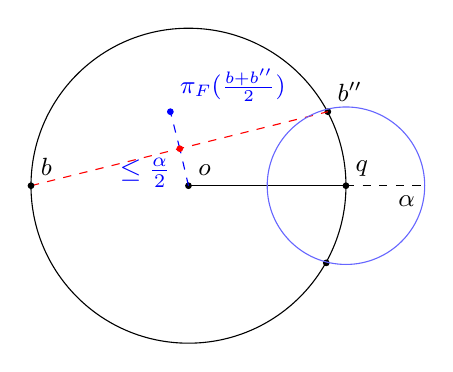
\begin{tikzpicture}

    \draw[color=black](0,0) circle (2);
  
    \filldraw[black] (0,0) circle (1pt) node[anchor=south west ]{\small $o$};
    \draw[black, thin] (0,0) -- (2,0) ;
    \filldraw[black] (1.77,0.94) circle (1pt) node[anchor=south west ]{\small $b''$};
    \draw[red, dashed] (-2,0) -- (1.77,0.94) node[anchor=north east ]{};
    \draw[blue, dashed] (0,0) -- (-0.11,0.47) node[anchor=north east ]{$\leq \frac{\alpha}{2}$};
    \draw[blue, dashed] (-0.11,0.47) -- (-0.23,0.94) node[anchor=north west ]{};
    \filldraw[blue] (-0.23,0.94) circle (1pt) node[anchor=south west ]{\small $\pi_F (\frac{b+b''}{2})$};
    \filldraw[red] (-0.11,0.47) circle (1pt) node[anchor=south east ]{};
    \filldraw[black] (1.75,-0.98) circle (1pt) node[anchor=south west ]{};
    \draw[color=blue!60, thin](2,0) circle (1);
    \filldraw[black] (2,0) circle (1pt) node[anchor=south west]{\small$q$};
    \draw[black, dashed] (2,0) -- (3,0) node[anchor=north east ]{ \small $\alpha$};
    % point(i)
    \filldraw[black] (-2,0) circle (1pt) node[anchor=south west]{\small $b$};
    % point(j)
\end{tikzpicture}
}
\newcommand{\tikzVI}{
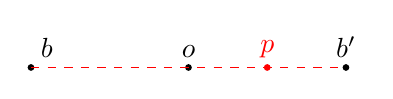
\begin{tikzpicture}

    \filldraw[black] (-2,0) circle (1pt) node[anchor=south west]{ $b$};
        \filldraw[black] (0,0) circle (1pt) node[anchor=south ]{ $o$};
        \filldraw[red] (1,0) circle (1pt) node[anchor=south ]{ $p$};
        \filldraw[black] (2,0) circle (1pt) node[anchor=south ]{ $b'$};
    \draw[red, dashed] (-2,0) -- (2,0) node[anchor=south  ]{};
    
    \end{tikzpicture}
}

\newcommand{\tikzVII}{
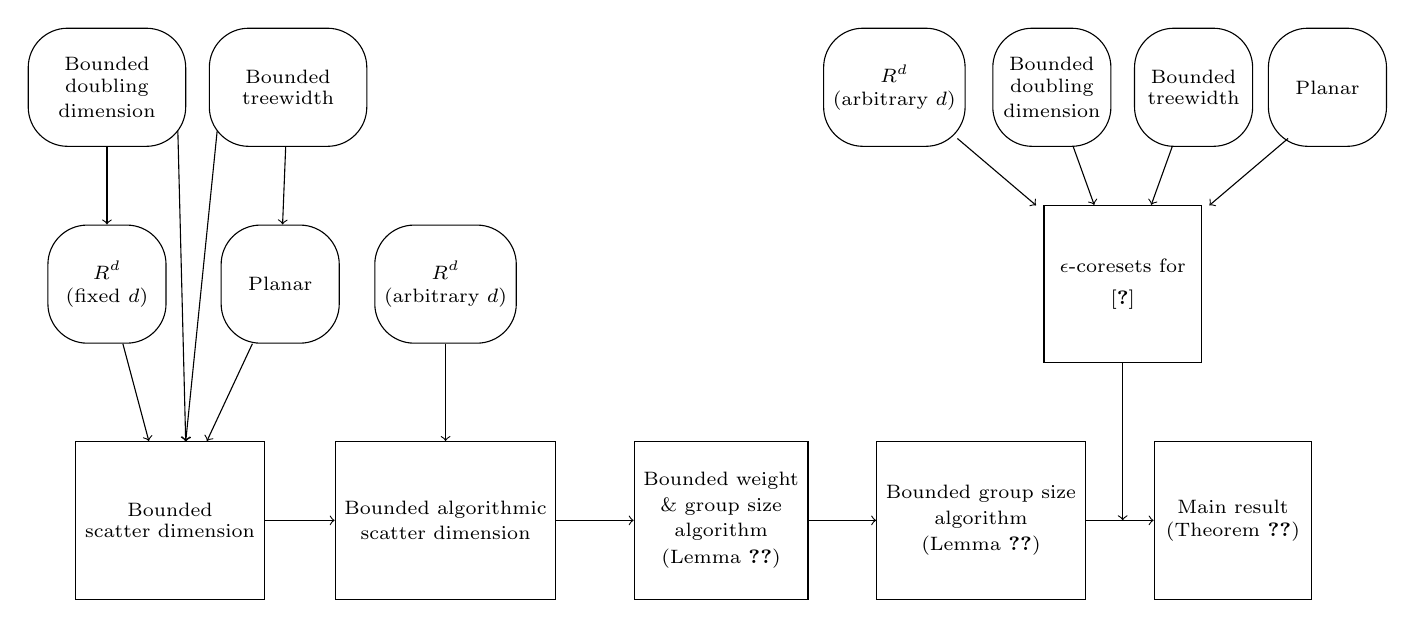
\begin{tikzpicture}
 %First Row
\tikzset{
LM/.style = {very thin,
        {Bar[]Stealth}-%
        {Stealth[]Bar}
            },
every edge quotes/.append style= {font=\footnotesize},
  every node/.append style ={font=\scriptsize} 
  }
 %%%%%% You can change the size of texts by above line


    \node[draw,
        minimum width=2cm,
        minimum height=2cm] (A) at (0.8,0) {\shortstack{ Bounded \\ scatter dimension}};
   
    \node[draw,
        minimum width=2cm,
        minimum height=2cm] (B) at (4.3,0) {\shortstack{ Bounded algorithmic\\scatter dimension}};
    \node[draw,
        minimum width=2cm,
        minimum height=2cm] (C) at (7.8,0) {\shortstack{ Bounded weight\\ \& group size\\
        algorithm\\(Lemma~\ref{lem:param-weights-size-kz})}};
    \node[draw,
        minimum width=2cm,
        minimum height=2cm] (D)  at (11.1,0) {\shortstack{ Bounded group size\\algorithm\\ (Lemma~\ref{lem:reduce-weights-kz})}};    
    \node[draw,
        minimum width=2cm,
        minimum height=2cm] (E) at (14.3,0) {\shortstack{ Main result\\ (Theorem~\ref{thm:mainer-kz})}};
% Second Row of The Chart
    \node[draw,
        rounded corners=0.5cm,
        minimum width=1.5cm,
        minimum height=1.5cm] (F) at (0,3) {\shortstack{$\mathbb{R}^d$\\(fixed $d$)}};
    \node[draw,
        rounded corners=0.5cm,
        minimum width=1.5cm,
        minimum height=1.5cm] (G) at (2.2,3) {\shortstack{ Planar}};
    \node[draw,
        rounded corners=0.5cm,
        minimum width=1.5cm,
        minimum height=1.5cm] (H)  at (4.3,3) {\shortstack{$\mathbb{R}^d$\\(arbitrary $d$)}};
    \node[draw,
        minimum width=2cm,
        minimum height=2cm] (J) at (12.9,3) {\shortstack{ $\epsilon$-coresets for\\ \kzc\\ \cite{cohen-addad-etal21:coreset-framework}}}; 
%Third Row of The chart
    \node[draw,
        rounded corners=0.5cm,
        minimum width=2cm,
        minimum height=1.5cm] (K) at (0,5.5) {\shortstack{ Bounded\\doubling\\ dimension}};
    \node[draw,
        rounded corners=0.5cm,
        minimum width=2cm,
        minimum height=1.5cm] (L) at (2.3,5.5) {\shortstack{ Bounded\\ treewidth}};
    \node[draw,
        rounded corners=0.5cm,
        minimum width=1.5cm,
        minimum height=1.5cm,black] (M) at (10,5.5){\shortstack{$\mathbb{R}^d$\\(arbitrary $d$)}};
    \node[draw,
        rounded corners=0.5cm,
        minimum width=1.5cm,
        minimum height=1.5cm,black] (W) at (12,5.5){\shortstack{Bounded\\doubling\\dimension}};        
    \node[draw,
        rounded corners=0.5cm,
        minimum width=1.5cm,
        minimum height=1.5cm,black] (N) at (13.8,5.5){\shortstack{Bounded\\treewidth}};
    \node[draw,
        rounded corners=0.5cm,
        minimum width=1.5cm,
        minimum height=1.5cm,black] (O) at (15.5,5.5){\shortstack{ Planar}};
        
 % here are the arrows to the boxes

   \path [->](A) edge (B);
   \path [->](B) edge (C);
   \path [->](C) edge (D);
   \path [->](D) edge (E);
   \path [->](F) edge (A);
   \path [->](G) edge (A);
   \path [->](H) edge (B);
   %\path [->](M) edge (J);
   \path [->](N) edge (J);
   %\path [->](O) edge (J);
   \path [->](W) edge (J);
   \path [->](L) edge (G);
   \path [->](K) edge (F);
% Extra  Lines are here
   \draw[black, thin, ->] (0.9,4.95) -- (1,1) ;
   \draw[black, thin, ->] (1.4,4.95) -- (1,1) ;
   \draw[black, thin, ->] (10.8,4.85) -- (11.8,4) ;
   \draw[black, thin, ->] (15,4.85) -- (14,4) ;
   \draw[black, thin, ->] (12.9,2) -- (12.9,0) ;
   %\draw[black, dotted, thick ] (11.95,5.5) -- (12.2,5.5) ;
      

\end{tikzpicture}
}

\newcommand{\tikzVIII}{
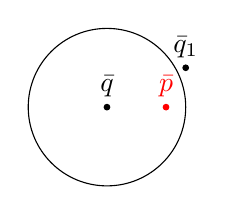
\begin{tikzpicture}
    \draw[color=black](0,0) circle (1);
     \filldraw[black] (0,0) circle (1pt) node[anchor=south ]{ $\bar q$};
     \filldraw[red] (0.75,0) circle (1pt) node[anchor=south ]{ $\bar p$};
    \filldraw[black] (1,0.5) circle (1pt) node[anchor=south ]{ $\bar q_1$};
    \end{tikzpicture}
}

\newcommand{\tikzIX}{
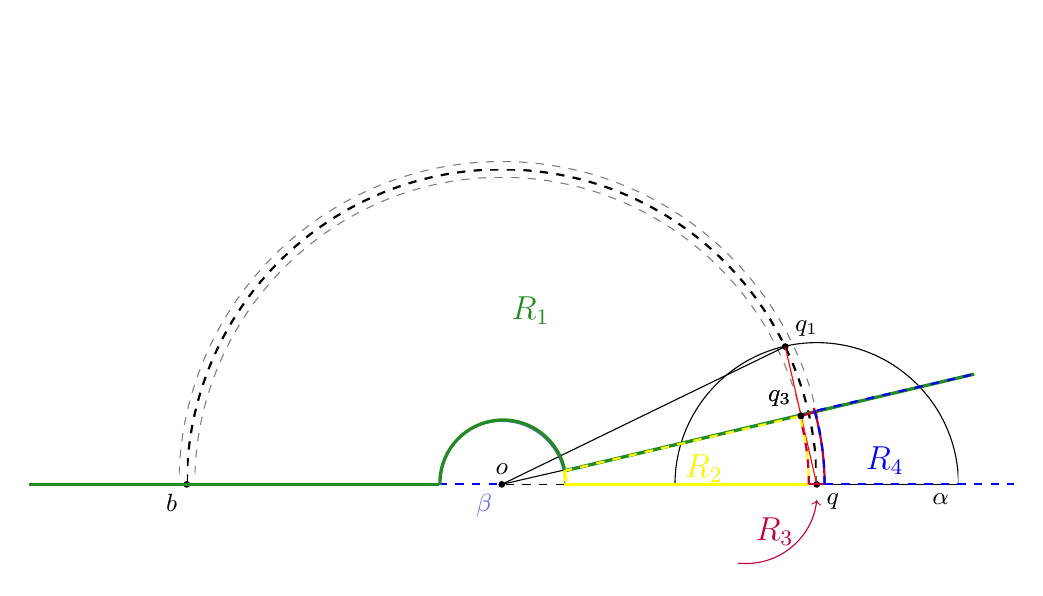
\begin{tikzpicture}
\begin{scope}

%  w-circle
    \clip (-4.1,0) rectangle (4.1,4.1);
    \draw[color=gray, dashed](0,0) circle (4.1);
    \clip (-4,0) rectangle (4,4);
% main circle
    \draw [color=black, dashed, thick](0,0) circle(4);
    \draw [color=black, dashed, thick] (-4,0) -- (4,0);
 % -w-circle
 
    \clip (-3.9,0) rectangle (3.9,3.9);
    \draw[color=gray, dashed](0,0) circle (3.9);
  % beta-circle 
    \clip (-0.8,0) rectangle (1,1);
    \draw[color=blue!60, inner color=white, thin](0,0) circle (0.8);
    \draw [color=blue, dashed, thick] (-0.8,0) -- (0,0);
% alpha circle

\end{scope}
\begin{scope}
   \clip (-2,0) rectangle (5.8,5.8);
    \draw[color=black, thin](4,0) circle (1.8);
\end{scope}
    \filldraw[black] (0,0) circle (1pt) node[anchor=south]{\small $o$};
    \draw[black, dashed] (1,0) -- (0,0) node[color=blue!60, anchor=north east]{\small $\beta$};
    % q and 1_1 and line between them 
    \filldraw[black] (4,0) circle (1pt) node[anchor=north west]{\small$q$};
    \filldraw[black] (3.6, 1.75) circle (1pt) node[anchor=south west]{\small$q_1$};
    \draw[red ] (4,0) -- ++(-0.4, 1.75); % Draw the line between q_1 and q
    \draw[black] (4,0) -- (5.8,0) node[anchor=north east]{\small $\alpha$};
    % point(i)
    \filldraw[black] (-4,0) circle (1pt) node[anchor=north east]{\small $b$};
    \draw[black] (0,0) -- (3.6, 1.75); % Draw the line between o and q_1

    \draw[black] (0,0) -- (3.8,0.875); % Draw the line between o and q_3 

%Region 1:
    \draw[ForestGreen, very thick] (0.79,0.17) -- (6,1.4) ;
    \draw[ForestGreen, very thick] (-0.8,0) -- (-6,0) ;
    \draw[ForestGreen, very thick] (0.8,0.17) arc (11:182:0.8);

% Region 2:
    \draw[Yellow,  thick, dashed] (0.79,0.17) -- (3.8,0.87) ;
    %\draw[ForestGreen, very thick] (1.87,0.49) -- (2,0) ;
    \draw[Yellow, very thick] (0.79,0) -- (3.9,0) ;
    \draw[Yellow,  thick] (3.9,0) arc (0:15.8:3.3);
    \draw[Yellow, very thick] (0.79,0.17) arc (28.2:-11.6:0.2);
    % point p_1

     \filldraw[black] (3.8,0.87) circle (1pt) node[anchor=south east]{\small$q_3$};
% Region 3:

    \draw[purple, thick] (3.9,0) -- (4.1,0) ;
    \draw[purple, thick] (3.8,0.87) -- (4.01,0.93) ;
    \draw[purple,  thick] (4.1,0) arc (0:16.10:3.5);
    \draw[purple, dashed, thick] (3.9,0) arc (0:15.8:3.3);

    % point p_1

     \filldraw[black] (3.8,0.87) circle (1pt) node[anchor=south east]{\small$q_3$};


% Region 4 
    \draw[blue , dashed, thick] (4.1,0) arc (0:16.10:3.5);
    \draw[blue , dashed, thick] (4.1,0) --(6.5,0);
    \draw[blue,dashed,  thick] (4.01,0.94) --(6,1.4);

    \filldraw[ForestGreen] (0,2.5)  node[anchor=north west]{\large $R_1$};

    \filldraw[yellow] (2.2,0.5)  node[anchor=north west]{\large $R_2$};

     \filldraw[blue] (4.5,0.6)  node[anchor=north west]{\large $R_4$};
      \draw[->, bend right=45, purple] (3,-1) to (4,-0.2) ;
    \filldraw[purple] (3.1,-0.3)  node[anchor=north west]{\large $R_3$};
\end{tikzpicture}


}